
%% Beginning of file 'sample63.tex'
%%
%% Modified 2019 June
%%
%% This is a sample manuscript marked up using the
%% AASTeX v6.3 LaTeX 2e macros.
%%
%% AASTeX is now based on Alexey Vikhlinin's emulateapj.cls 
%% (Copyright 2000-2015).  See the classfile for details.

%% AASTeX requires revtex4-1.cls (http://publish.aps.org/revtex4/) and
%% other external packages (latexsym, graphicx, amssymb, longtable, and epsf).
%% All of these external packages should already be present in the modern TeX 
%% distributions.  If not they can also be obtained at www.ctan.org.

%% The first piece of markup in an AASTeX v6.x document is the \documentclass
%% command. LaTeX will ignore any data that comes before this command. The 
%% documentclass can take an optional argument to modify the output style.
%% The command below calls the preprint style which will produce a tightly 
%% typeset, one-column, single-spaced document.  It is the default and thus
%% does not need to be explicitly stated.
%%
%%
%% using aastex version 6.3
\documentclass{aastex63}

%% The default is a single spaced, 10 point font, single spaced article.
%% There are 5 other style options available via an optional argument. They
%% can be invoked like this:
%%
%% \documentclass[arguments]{aastex63}
%% 
%% where the layout options are:
%%
%%  twocolumn   : two text columns, 10 point font, single spaced article.
%%                This is the most compact and represent the final published
%%                derived PDF copy of the accepted manuscript from the publisher
%%  manuscript  : one text column, 12 point font, double spaced article.
%%  preprint    : one text column, 12 point font, single spaced article.  
%%  preprint2   : two text columns, 12 point font, single spaced article.
%%  modern      : a stylish, single text column, 12 point font, article with
%% 		  wider left and right margins. This uses the Daniel
%% 		  Foreman-Mackey and David Hogg design.
%%  RNAAS       : Preferred style for Research Notes which are by design 
%%                lacking an abstract and brief. DO NOT use \begin{abstract}
%%                and \end{abstract} with this style.
%%
%% Note that you can submit to the AAS Journals in any of these 6 styles.
%%
%% There are other optional arguments one can invoke to allow other stylistic
%% actions. The available options are:
%%
%%   astrosymb    : Loads Astrosymb font and define \astrocommands. 
%%   tighten      : Makes baselineskip slightly smaller, only works with 
%%                  the twocolumn substyle.
%%   times        : uses times font instead of the default
%%   linenumbers  : turn on lineno package.
%%   trackchanges : required to see the revision mark up and print its output
%%   longauthor   : Do not use the more compressed footnote style (default) for 
%%                  the author/collaboration/affiliations. Instead print all
%%                  affiliation information after each name. Creates a much 
%%                  longer author list but may be desirable for short 
%%                  author papers.
%% twocolappendix : make 2 column appendix.
%%   anonymous    : Do not show the authors, affiliations and acknowledgments 
%%                  for dual anonymous review.
%%
%% these can be used in any combination, e.g.
%%
%% \documentclass[twocolumn,linenumbers,trackchanges]{aastex63}
%%
%% AASTeX v6.* now includes \hyperref support. While we have built in specific
%% defaults into the classfile you can manually override them with the
%% \hypersetup command. For example,
%%
%% \hypersetup{linkcolor=red,citecolor=green,filecolor=cyan,urlcolor=magenta}
%%
%% will change the color of the internal links to red, the links to the
%% bibliography to green, the file links to cyan, and the external links to
%% magenta. Additional information on \hyperref options can be found here:
%% https://www.tug.org/applications/hyperref/manual.html#x1-40003
%%
%% Note that in v6.3 "bookmarks" has been changed to "true" in hyperref
%% to improve the accessibility of the compiled pdf file.
%%
%% If you want to create your own macros, you can do so
%% using \newcommand. Your macros should appear before
%% the \begin{document} command.
%%
\newcommand{\vdag}{(v)^\dagger}
\newcommand\aastex{AAS\TeX}
\newcommand\latex{La\TeX}

%% Reintroduced the \received and \accepted commands from AASTeX v5.2
\received{June 1, 2019}
\revised{January 10, 2019}
\accepted{\today}
%% Command to document which AAS Journal the manuscript was submitted to.
%% Adds "Submitted to " the argument.
\submitjournal{AJ}

%% For manuscript that include authors in collaborations, AASTeX v6.3
%% builds on the \collaboration command to allow greater freedom to 
%% keep the traditional author+affiliation information but only show
%% subsets. The \collaboration command now must appear AFTER the group
%% of authors in the collaboration and it takes TWO arguments. The last
%% is still the collaboration identifier. The text given in this
%% argument is what will be shown in the manuscript. The first argument
%% is the number of author above the \collaboration command to show with
%% the collaboration text. If there are authors that are not part of any
%% collaboration the \nocollaboration command is used. This command takes
%% one argument which is also the number of authors above to show. A
%% dashed line is shown to indicate no collaboration. This example manuscript
%% shows how these commands work to display specific set of authors 
%% on the front page.
%%
%% For manuscript without any need to use \collaboration the 
%% \AuthorCollaborationLimit command from v6.2 can still be used to 
%% show a subset of authors.
%
%\AuthorCollaborationLimit=2
%
%% will only show Schwarz & Muench on the front page of the manuscript
%% (assuming the \collaboration and \nocollaboration commands are
%% commented out).
%%
%% Note that all of the author will be shown in the published article.
%% This feature is meant to be used prior to acceptance to make the
%% front end of a long author article more manageable. Please do not use
%% this functionality for manuscripts with less than 20 authors. Conversely,
%% please do use this when the number of authors exceeds 40.
%%
%% Use \allauthors at the manuscript end to show the full author list.
%% This command should only be used with \AuthorCollaborationLimit is used.

%% The following command can be used to set the latex table counters.  It
%% is needed in this document because it uses a mix of latex tabular and
%% AASTeX deluxetables.  In general it should not be needed.
%\setcounter{table}{1}

%%%%%%%%%%%%%%%%%%%%%%%%%%%%%%%%%%%%%%%%%%%%%%%%%%%%%%%%%%%%%%%%%%%%%%%%%%%%%%%%
%%
%% The following section outlines numerous optional output that
%% can be displayed in the front matter or as running meta-data.
%%
%% If you wish, you may supply running head information, although
%% this information may be modified by the editorial offices.
\shorttitle{Of Dust Devils and Diameters}
\shortauthors{Jackson}
%%
%% You can add a light gray and diagonal water-mark to the first page 
%% with this command:
%% \watermark{text}
%% where "text", e.g. DRAFT, is the text to appear.  If the text is 
%% long you can control the water-mark size with:
%% \setwatermarkfontsize{dimension}
%% where dimension is any recognized LaTeX dimension, e.g. pt, in, etc.
%%
%%%%%%%%%%%%%%%%%%%%%%%%%%%%%%%%%%%%%%%%%%%%%%%%%%%%%%%%%%%%%%%%%%%%%%%%%%%%%%%%
\graphicspath{{./}{figures/}}
%% This is the end of the preamble.  Indicate the beginning of the
%% manuscript itself with \begin{document}.

\usepackage{amsmath}
\usepackage{amssymb}

\begin{document}

\title{Of Dust Devils and Diameters}

%% LaTeX will automatically break titles if they run longer than
%% one line. However, you may use \\ to force a line break if
%% you desire. In v6.3 you can include a footnote in the title.

%% A significant change from earlier AASTEX versions is in the structure for 
%% calling author and affiliations. The change was necessary to implement 
%% auto-indexing of affiliations which prior was a manual process that could 
%% easily be tedious in large author manuscripts.
%%
%% The \author command is the same as before except it now takes an optional
%% argument which is the 16 digit ORCID. The syntax is:
%% \author[xxxx-xxxx-xxxx-xxxx]{Author Name}
%%
%% This will hyperlink the author name to the author's ORCID page. Note that
%% during compilation, LaTeX will do some limited checking of the format of
%% the ID to make sure it is valid. If the "orcid-ID.png" image file is 
%% present or in the LaTeX pathway, the OrcID icon will appear next to
%% the authors name.
%%
%% Use \affiliation for affiliation information. The old \affil is now aliased
%% to \affiliation. AASTeX v6.3 will automatically index these in the header.
%% When a duplicate is found its index will be the same as its previous entry.
%%
%% Note that \altaffilmark and \altaffiltext have been removed and thus 
%% can not be used to document secondary affiliations. If they are used latex
%% will issue a specific error message and quit. Please use multiple 
%% \affiliation calls for to document more than one affiliation.
%%
%% The new \altaffiliation can be used to indicate some secondary information
%% such as fellowships. This command produces a non-numeric footnote that is
%% set away from the numeric \affiliation footnotes.  NOTE that if an
%% \altaffiliation command is used it must come BEFORE the \affiliation call,
%% right after the \author command, in order to place the footnotes in
%% the proper location.
%%
%% Use \email to set provide email addresses. Each \email will appear on its
%% own line so you can put multiple email address in one \email call. A new
%% \correspondingauthor command is available in V6.3 to identify the
%% corresponding author of the manuscript. It is the author's responsibility
%% to make sure this name is also in the author list.
%%
%% While authors can be grouped inside the same \author and \affiliation
%% commands it is better to have a single author for each. This allows for
%% one to exploit all the new benefits and should make book-keeping easier.
%%
%% If done correctly the peer review system will be able to
%% automatically put the author and affiliation information from the manuscript
%% and save the corresponding author the trouble of entering it by hand.

\correspondingauthor{Brian Jackson}
\email{bjackson@boisestate.edu}

\author[0000-0002-9495-9700]{Brian Jackson}
\affiliation{Boise State University, Dept.~of Physics\\
1910 University Drive, Boise ID 83725-1570}

%% Note that the \and command from previous versions of AASTeX is now
%% depreciated in this version as it is no longer necessary. AASTeX 
%% automatically takes care of all commas and "and"s between authors names.

%% AASTeX 6.3 has the new \collaboration and \nocollaboration commands to
%% provide the collaboration status of a group of authors. These commands 
%% can be used either before or after the list of corresponding authors. The
%% argument for \collaboration is the collaboration identifier. Authors are
%% encouraged to surround collaboration identifiers with ()s. The 
%% \nocollaboration command takes no argument and exists to indicate that
%% the nearby authors are not part of surrounding collaborations.

%% Mark off the abstract in the ``abstract'' environment. 
\begin{abstract}

Words

\end{abstract}

%% Keywords should appear after the \end{abstract} command. 
%% See the online documentation for the full list of available subject
%% keywords and the rules for their use.
\keywords{editorials, notices --- 
miscellaneous --- catalogs --- surveys}

%% From the front matter, we move on to the body of the paper.
%% Sections are demarcated by \section and \subsection, respectively.
%% Observe the use of the LaTeX \label
%% command after the \subsection to give a symbolic KEY to the
%% subsection for cross-referencing in a \ref command.
%% You can use LaTeX's \ref and \label commands to keep track of
%% cross-references to sections, equations, tables, and figures.
%% That way, if you change the order of any elements, LaTeX will
%% automatically renumber them.
%%
%% We recommend that authors also use the natbib \citep
%% and \citet commands to identify citations.  The citations are
%% tied to the reference list via symbolic KEYs. The KEY corresponds
%% to the KEY in the \bibitem in the reference list below. 

\section{Model} \label{sec:model}

At the dust devil's eyewall, the pressure gradient force balance the centrifugal force:
\begin{equation}
    \dfrac{1}{\rho}\left( \dfrac{dp}{dr} \right) = \dfrac{\upsilon^2}{R},
\end{equation}
where $\rho$ is the density, $p$ the pressure, $r$ radial distance from the devil's center, $\upsilon$ the tangential velocity, and $R$ the devil's eyewall radius. 

Dust devils have pressure structures resembling a Lorentz profile:
\begin{equation}
    p(r) = p_{\infty} - \dfrac{\Delta p}{1 + \left( ^r/_R \right)^2},\label{eqn:pressure_profile}
\end{equation}
where $p_{\infty}$ is the ambient pressure, and $\Delta p$ is the depth of the pressure perturbation at the devil's center.

Calculating the pressure gradient from this profile and equating it to the centrifugal acceleration at $r = R$ gives
\begin{equation}
    \dfrac{\Delta p}{2\rho} = \upsilon^2.\label{eqn:cyclostrophic_balance}
\end{equation}

The dust devil's pressure gradient influences the wind field and draws in air out to a distance $r = r_{\rm inf} = n R$, i.e. some number of dust devil radii out. In the presence of wind shear $\partial U/\partial x \equiv \alpha$, drawing in air from $r_{\rm inf}$ also brings in a specific angular momentum $l \approx \alpha\ r_{\rm inf}^2$. Assuming this angular momentum is conserved as the fluid travels from $r_{\rm inf}$ to $R$ implies $\alpha\ r_{\rm inf}^2 = \alpha\ n^2 R^2 \approx \upsilon\ R$ or 
\begin{equation}
    \upsilon \approx \alpha n^2 R
\end{equation}

Using Equation \ref{eqn:cyclostrophic_balance}, we find
\begin{equation}
    R \approx \alpha^{-1} n^{-2} \left( \dfrac{\Delta p}{\rho} \right)^{1/2},\label{eqn:R_vs_Delta-p}
\end{equation}
neglecting terms of order unity. This equation suggests the perhaps counter-intuitive result that $R$ \emph{decreases} with increasing angular momentum, $l$. However, larger $l$ also implies a larger centrifugal force at the devil eyewall. $R$ sets the magnitude of the pressure gradient at a given distance $r$, so a smaller $R$ provides the larger gradient required to balance the centrifugal force.

Next, we can express the radius in terms of the dust devil height $h$. \citet{1998JAtS...55.3244R} suggests
\begin{equation}
    \Delta p = p_{\infty} \left\{ 1 - \exp \left[ \left( \dfrac{\gamma \eta}{\gamma \eta - 1}\right) \left(\dfrac{1}{\chi}\right) \left( \dfrac{\Delta T}{T_{\infty}}\right) \right] \right\}\label{eqn:Renno_Delta-p},
\end{equation}{}
where $\chi$ is the ratio of the gas constant $R_\star$ to the specific heat capacity at constant pressure $c_{\rm p}$, $\gamma$ is the fraction of total dissipation of mechanical within the dust devil consumed by friction near the surface, and $\Delta T$ the difference in temperature between the positive perturbation at the devil's center and the ambient temperature $T_\infty$. $\eta$ is the thermodynamic efficiency and is given by 
\begin{equation}
    \eta = \dfrac{T_{\rm h} - T_{\rm c}}{T_{\rm h}}\label{eqn:Renno_eta},
\end{equation}{}
where $T_{\rm h}$ is the entropy-weighted mean temperature near the surface where heat is absorbed, and $T_{\rm c}$ is the same for the cold sink at the top of the dust devil. Estimates of $\eta$ based on field observations suggest $\eta \lesssim 0.1$ \citep[e.g.][]{2000JGR...105.1859R}. A useful approximation gives $T_{\rm h} \approx T_\infty$, while
\begin{equation}
    T_{\rm c} = \left[ \dfrac{ p_\infty^{\chi + 1} - p_{c}^{\chi + 1} }{\left( p_\infty - p_{c} \right) \left( \chi + 1\right) p_\infty^{\chi}} \right] T_{\rm h},\label{eqn:Tc}
\end{equation}{} 
$p_{\rm c}$ is the pressure near the top of the dust devil and is related to the surface pressure as $p_{\rm c} \approx p_\infty \exp\left(-h/H\right)$, where $h$ is the height of the dust devil and $H$ is the atmospheric scale height. For Mars, $H \ge 10\,{\rm km}$, and, although dust devils are sometimes observed that tall, usually they are a few km or less in height \citep{2008Icar..197...39S}. 

We can plug these expressions into Equation \ref{eqn:Renno_eta} and expand about small $h/H$:
\begin{equation}
    \eta \approx \frac{1}{2} \chi \left( \dfrac{h}{H} \right).\label{eqn:approx_eta}
\end{equation}{}

\begin{figure}
    \centering
    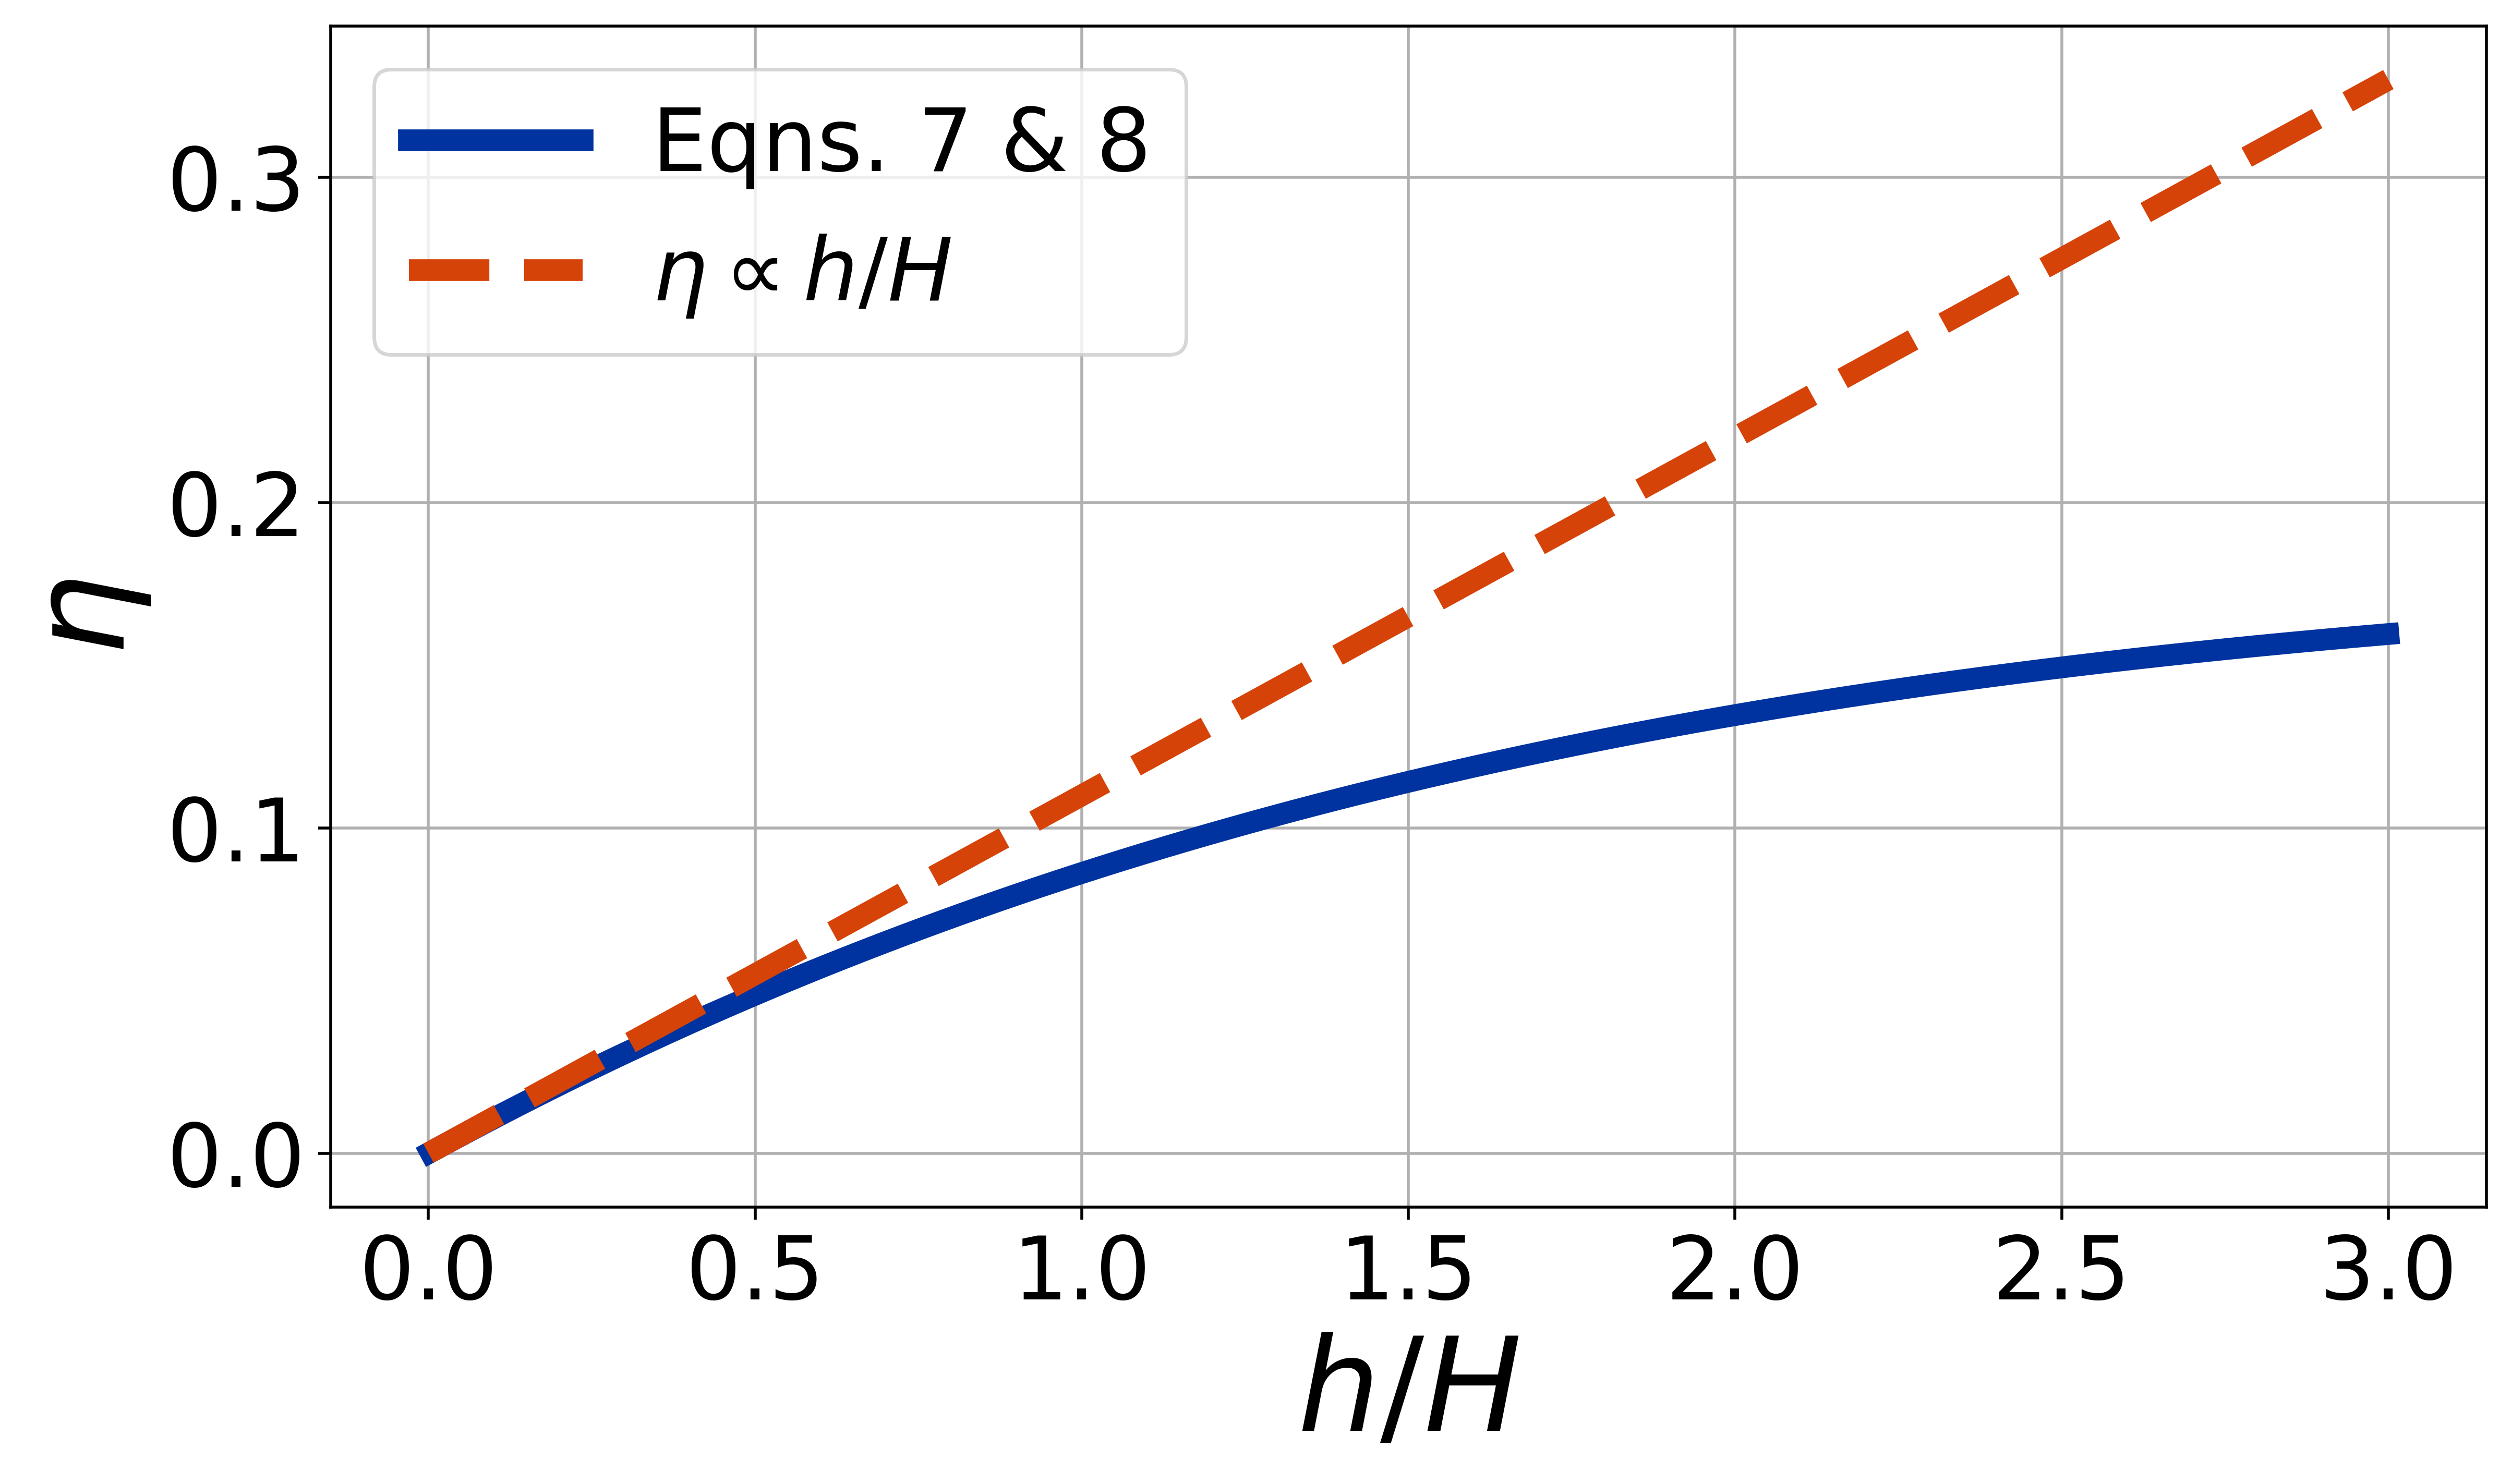
\includegraphics[width=\textwidth]{eta_vs_h-over-H.png}
    \caption{Dust devil thermodynamic efficiency $\eta$ as a function of dust devil height $h$ normalized to the atmospheric scale height $H$. The solid, blue line shows the full behavior given by Equations \ref{eqn:Renno_eta} and \ref{eqn:Tc}, while the dashed, orange line shows a linear approximation.}
    \label{fig:eta_vs_h-over-H}
\end{figure}{}

In other words, for relatively short dust devils, the thermodynamic efficiency increases linearly with their heights. Figure \ref{fig:eta_vs_h-over-H} shows the resulting dependence of $\eta$ on $h/H$ for arbitrary values and confirms the linear behavior for small $h/H$. We can plug Equation \ref{eqn:approx_eta} into Equation \ref{eqn:Renno_Delta-p} and expand about small $h/H$, giving
\begin{equation}
    \Delta p \approx \left( \dfrac{\gamma R_\star \rho \Delta T}{2} \right) \left( \dfrac{h}{H} \right) \label{eqn:approx_Delta-p},
\end{equation}
with $p_\infty T_\infty = R_\star \rho$.

Since their radii $R$ depend on the scale of the pressure perturbation, which itself depends on $\eta$, we can write a relationship between $R$ and $h$:
\begin{equation}
    R \approx \alpha^{-1} n^{-1} \left( \dfrac{\gamma R_\star \Delta T}{H} \right)^{1/2}\ h^{1/2},\label{eqn:R_vs_h}
\end{equation}{}
with factors of order unity neglected.



\bibliography{sample63}
\bibliographystyle{aasjournal}

%% This command is needed to show the entire author+affiliation list when
%% the collaboration and author truncation commands are used.  It has to
%% go at the end of the manuscript.
%\allauthors

%% Include this line if you are using the \added, \replaced, \deleted
%% commands to see a summary list of all changes at the end of the article.
%\listofchanges

\end{document}

% End of file `sample63.tex'.
